% AI6102 Team Project report: Kaggle "Name That LLM" (ongoing competition).
% Build: tectonic main.tex   (figures: report/figures/make_figures.py)
\documentclass[10pt,twocolumn,letterpaper]{article}
\usepackage[top=1in,bottom=1in,left=0.8125in,right=0.8125in,columnsep=0.3125in]{geometry}
\usepackage{times}
\usepackage[T1]{fontenc}
\usepackage{amsmath,amssymb}
\usepackage{graphicx}
\usepackage{booktabs}
\usepackage{multirow}
\usepackage{xcolor}
\usepackage{enumitem}
\usepackage[font=small,labelfont=bf,skip=4pt]{caption}
\usepackage[hidelinks]{hyperref}
\usepackage{xurl}
\setlist{nosep,leftmargin=*}
\setlength{\tabcolsep}{4pt}
\setlength{\emergencystretch}{1.5em}
\newcommand{\todo}[1]{\textcolor{red}{[TODO: #1]}}
\newcommand{\BA}{\mathrm{BA}}

\title{\vspace{-0.6cm}Who Wrote This Paragraph?\\Exact-Model LLM Attribution under Prompt Shift}
\author{
Bao Ning\\[4pt]
\small AI6102 Team Project (individual) --- ongoing Kaggle competition \emph{Name That LLM} (Kaggle team \emph{Monte Carlo})
}
\date{\vspace{-0.8cm}}

\begin{document}
\maketitle

\begin{abstract}
\emph{Name That LLM} is an ongoing Kaggle competition: given one paragraph, name which of 18 large language models wrote it. Many of the 18 are close siblings from the same provider. Submissions are scored by balanced accuracy (BA) on about 4,000 hidden passages written for prompts that never appear in training. Only 150 prompts with 18 labelled answers each are provided. We built a nested, prompt-grouped validation protocol with a locked confirmation set, and used it to test a sequence of models: a stylometric linear baseline (0.355 CV BA), fine-tuned encoders, two-stage training on a 212k-passage community corpus, and finally a truncated, multi-depth-pooled Qwen3-8B LoRA classifier. That last model scores 0.623 in nested CV and 0.633 on the locked confirmation prompts. With test-time soft centring it reaches 0.619 on the public leaderboard. Data drove most of the progress: pool pre-training added +0.14 BA to the same encoder, while architecture changes, ensembling, sibling-focused training and dedicated within-provider specialists each added 0.01 or less. Word-choice fingerprints are strong between providers and model generations, but close siblings show none. Our best model gets the provider family right on 85\% of passages, so most remaining errors are confusions between sibling models. We analyse why we plateaued about 0.085 below the best public notebook (0.704) and 0.14 below the top ten. The causes we identify are training data that does not match the hosts' generation setup, an intrinsic sibling-confusion ceiling, ensemble members that make the same mistakes, a test layout that grouped CV does not reproduce, and compute limits.
\end{abstract}

%=====================================================================
\section{Problem statement}
\label{sec:problem}

The competition asks a forensic question about machine-generated text. Each sample is a single English paragraph (36--274 words, median 101) written by one of 18 chat models: five Anthropic models (\texttt{claude-fable-5}, \texttt{claude-opus-4-6}, \texttt{-4-8}, \texttt{claude-opus-5}, \texttt{claude-sonnet-5}), four Google models (\texttt{gemini-3.1-pro-preview}, \texttt{3.6/3.7/3.8-flash}), two from Z.ai (\texttt{glm-5.3}, \texttt{glm-5.3-flash}), five from OpenAI (\texttt{gpt-5.5}, \texttt{gpt-5.6-luna/sol/terra}, \texttt{gpt-6-astra}), and \texttt{kimi-k3} and \texttt{qwen3.8-max}. The task is to predict the exact model, not just its provider.

The training set has 2,699 passages: 150 prompts, each answered once by every model (one cell, \texttt{p002}/\texttt{claude-fable-5}, is missing). The hidden test set holds about 4,000 passages for \emph{new} prompts. Its class mixture is unequal and differs between the public and private splits, and it carries no prompt identifier. The metric is balanced accuracy, $\BA = \frac{1}{18}\sum_{c} \mathrm{recall}_c$~\cite{brodersen2010}, so every model counts equally however rare it is in the test. Inference runs in an offline Kaggle notebook (two T4 GPUs, a 9-hour limit) that must read \texttt{test.csv} and write \texttt{submission.parquet}.

Our framing is supervised 18-way classification under \emph{covariate shift across prompts}. A model must learn each author's habits (typography, word choice, rhythm, structure), and those habits must transfer to topics it has never seen. This is authorship attribution~\cite{stamatatos2009} for neural text~\cite{uchendu2020}. It is harder than detecting AI text~\cite{mitchell2023detectgpt,bao2024fastdetectgpt}, because every candidate author is an LLM and several of them share training lineage.

%=====================================================================
\section{Challenges}
\label{sec:challenges}

\begin{enumerate}[label=\textbf{C\arabic*},leftmargin=2.2em,labelsep=0.5em]
\item \textbf{Sibling models.} Models from one provider share tokenizers, post-training data and house style. Gemini~3.7 and 3.8 Flash, or the three \texttt{gpt-5.6} variants, differ in subtle frequencies, not in any single marker (\S\ref{sec:why}).
\item \textbf{Prompt shift and topic confounding.} All 18 answers to one prompt share their content. A classifier that memorises topic--author co-occurrences looks good under random splits and fails on new prompts, so validation must be grouped by prompt.
\item \textbf{Very little labelled data.} There are 150 prompts and 2,699 rows. Our learning curve (Fig.~\ref{fig:scaling}a) is still rising at 96 training prompts.
\item \textbf{Unknown generation setup.} Hosts used particular API versions, system prompts and decoding settings, and possibly cleaned the output. New data generated by others (or by us) can differ in style from the official rows. One example: official Gemini text has an em dash in 1 of 600 passages, while our own Gemini API answers have one in 21--35\%. \texttt{gemini-3.7-flash} can no longer be requested at all, because Google now routes it to 3.8.
\item \textbf{A test set unlike the training layout.} The test has unequal, unknown class priors and, according to community analysis, only about two answers per prompt. Tricks that exploit all 18 answers per prompt in CV therefore do not transfer. The public leaderboard scores about 40\% of the test, and identical code is reported to vary by up to $\pm$0.009 between submissions.
\item \textbf{Compute.} Our training budget was one shared L40S (46\,GB) on the NTU TC2 cluster (5\,h\,50\,min per job, at most two jobs on a shared account) and a 16\,GB RTX 5070 Ti workstation. Inference had to fit two T4s in the Kaggle notebook.
\end{enumerate}

%=====================================================================
\section{Data analysis and motivation}
\label{sec:motivation}

\begin{table}[t]
\centering\small
\caption{Share of official passages containing each marker, by provider (all 150 prompts). Typography separates families strongly. Note Google's near-total absence of em dashes, and Anthropic/Z.ai's absence of curly apostrophes.}
\label{tab:typo}
\setlength{\tabcolsep}{3.5pt}
\begin{tabular}{lccccc}
\toprule
Provider & Em dash & Curly ' & Straight \textquotesingle & Semicol. & Words \\
\midrule
Anthropic (5) & 0.75 & 0.00 & 0.63 & 0.30 & 119 \\
Google (4) & \textbf{0.00} & 0.20 & 0.14 & 0.23 & 112 \\
Z.ai (2) & 0.81 & 0.00 & 0.63 & 0.41 & 115 \\
OpenAI (5) & 0.22 & 0.47 & 0.05 & 0.54 & 115 \\
Moonshot (1) & 0.52 & 0.32 & 0.23 & 0.61 & 107 \\
Qwen (1) & 0.03 & 0.29 & 0.12 & 0.39 & 108 \\
\bottomrule
\end{tabular}
\end{table}

\paragraph{Typography is the strongest single cue, so we never normalise text.} Table~\ref{tab:typo} shows marker rates that separate the providers almost categorically. Lowercasing, Unicode NFKC or quote folding would erase this signal. Every model therefore reads the raw string. We also avoided scikit-learn's \texttt{char} analyser, which collapses whitespace, in favour of a custom byte-faithful n-gram extractor. We did not use paraphrase or translation augmentation, since either would change the very style we classify.

\paragraph{Family is easier than version.} Anthropic and Z.ai share the em-dash / straight-apostrophe profile, and Z.ai's \texttt{glm-5.3} is often mistaken for \texttt{claude-fable-5}. Within a family the markers barely differ. This shaped two choices: classifiers that see whole sequences (encoders and decoders) rather than marker counts alone, and a strong interest in data that matches each model's exact serving setup.

\paragraph{Prompt grouping is part of the problem.} Answers to the same prompt share an offset in any model's score space, namely the topic. That motivated the prompt-triplet ``centred'' head in training and soft centring within inferred prompt clusters at test time (\S\ref{sec:centring}).

\paragraph{Word choice is a fingerprint too.} Beyond punctuation, models prefer particular words (Table~\ref{tab:words}). To make sure these are habits rather than topic, we found each label's over- and under-used words and sentence openers in 168k community passages, taken from prompts answered by at least six labels so that topic is shared. We then tested them on the 150 official prompts, where every label answers every prompt. For 17 of the 18 labels, 76--100\% of the pool's top 80 tokens point the same way on official text; each Gemini label has 32--48 of its 80 confirmed at $z\geq3$. The families have recognisable registers. Gemini writes dramatically and avoids hedges. GPT reasons in hedged connectives. Claude is the most conversational. GLM leans on absolutes and negation, and \texttt{claude-fable-5} shares that vocabulary, which is consistent with the GLM/fable confusion in Fig.~\ref{fig:confusion}.

\begin{table*}[t]
\centering\small
\caption{Word-choice fingerprints found in the community pool and confirmed on official text. Numbers are the share of official passages using the word: this label vs all other labels (\%). ``Opens'' means the word starts a sentence.}
\label{tab:words}
\begin{tabular}{p{2.6cm}p{9.2cm}p{4.4cm}}
\toprule
Group & Over-uses & Avoids \\
\midrule
Gemini (all four) & \emph{profound} (3.1-pro 22 vs 3), \emph{vibrant}, \emph{sprawling}, \emph{suffocating}, \emph{colossal}, \emph{relentless}, \emph{perpetual}, \emph{seamlessly}; opens with \emph{Ultimately}, \emph{Conversely}, \emph{Consequently}, \emph{Instead} & \emph{may} (1--3 vs 12), \emph{still} (1--3 vs 13), \emph{then}, \emph{each}, \emph{than}, \emph{what}, \emph{one} \\
GPT & \emph{may} (luna 25, terra 24 vs 11), \emph{therefore}/\emph{thus} (luna 14 vs 4), \emph{not merely} (terra 16 vs 7); gpt-5.5: \emph{like} (53 vs 31), \emph{as if}; gpt-6-astra: \emph{help}, \emph{although}, \emph{not simply}, \emph{need not}, \emph{familiar} & gpt-5.5: \emph{this} (20 vs 41), \emph{these} \\
Claude & sonnet-5: contractions \emph{isn't}, \emph{it's}, \emph{doesn't} (4--5 vs 1), \emph{actually}, \emph{just}; opus-5: \emph{thing}, \emph{which is}, opens with \emph{And}/\emph{So}; opus-4-6: \emph{cathedral} (8 vs 2) & opus-5: \emph{ancient} (1 vs 13), \emph{human}, \emph{these} \\
GLM (both) and claude-fable-5 & \emph{nothing} (15--17 vs 8), \emph{itself} (28--31 vs 18), \emph{never} (GLM 24--25 vs 14), \emph{at all}, \emph{no one}; fable also \emph{everything} & fable: \emph{not} (32 vs 45) \\
Kimi, Qwen & Kimi: \emph{becomes} (23 vs 14), \emph{keeps}; Qwen: \emph{luminous} (13 vs 4), \emph{turning}, \emph{becomes a}, \emph{memory}; opens with \emph{Each} & \emph{an} (24--27 vs 42); Kimi also \emph{of} \\
\bottomrule
\end{tabular}
\end{table*}

%=====================================================================
\section{Proposed solution}
\label{sec:method}

\subsection{Validation protocol}
\label{sec:validation}
Before training any model we froze a split plan. The 150 prompts were divided into 30 \emph{locked confirmation} prompts, to be scored exactly once on the final recipe, and 120 \emph{development} prompts. The development prompts were split twice (two \emph{partitions}) into 5 outer folds of 96 train / 24 validation prompts, and each outer training set into 3 inner folds of 64/32. Everything learned (vectoriser vocabularies, scalers, epochs, learning rates, blend weights, calibration) was chosen on inner out-of-fold (OOF) predictions only. The outer validation prompts were only scored, so the reported number is the concatenated outer-fold BA over all 120 development prompts. This nested design avoids the optimistic bias of selecting and evaluating on the same folds~\cite{varma2006}. We report 95\% \emph{prompt-cluster} bootstrap intervals (2,000 resamples of whole prompts~\cite{efron1993}), and we promote a change only if its \emph{paired} bootstrap difference has a lower bound above zero on both partitions.

\subsection{Stage A: stylometric linear baseline}
Two linear branches. (i) \emph{Text}: raw character 3--5 or 2--6-grams plus case-preserving word 1--2-grams in which every punctuation mark is a token, each TF-IDF weighted (raw or sublinear TF), fed to logistic regression or a linear SVM. (ii) \emph{Style}: 51 numeric features (marker rates, sentence and word lengths, punctuation density) with logistic regression or gradient-boosted trees. The two branches' decision scores are standardised and blended with a weight chosen on inner folds.

\subsection{Stage B: fine-tuned encoders}
We fully fine-tune Ettin-400M~\cite{weller2025ettin} (a ModernBERT-style encoder~\cite{warner2024modernbert}), Ettin-1B and RoBERTa-large~\cite{liu2019roberta} with mean pooling and a linear head. Settings: cross-entropy, AdamW~\cite{loshchilov2019}, bf16, maximum length 512, effective batch 32, linear warmup and decay. Each fit records held-out logits after every epoch, so the epoch is selected on inner folds at no extra cost.

\subsection{External training data}
\label{sec:external}
\textbf{Own collection.} Following provenance rules (one fresh conversation per prompt, nothing edited, no model asked to identify itself), we built a bank of 196 new prompts and collected 4,828 answers from all 18 models' chat products, APIs and agent CLIs. \textbf{Community pool.} We also used \emph{Open Pool v13}~\cite{kaggle_pool}, a community Kaggle dataset of 190,588 passages generated by many teams for the 18 labels on about 31k prompts, plus 21k cleaned rows from two further CC-BY datasets. Every external row was filtered to exclude near-duplicates of official text (TF-IDF cosine $<0.3$).

\textbf{Match weights.} The pool's style drifts from official text, for example in length and dash rates. So, inside each fold, we reweight pool rows per label by exponential tilting, such that 15 marker rates and 4 length bins match that fold's official training rows (ridge 0.02). \textbf{Two-stage training.} Stage~1 trains on class-balanced pool rows. Stage~2 continues on the official training prompts, using the nested selection above.

\subsection{Stage C: decoder classifier (Qwen3-8B LoRA24)}
Our first decoder followed the usual recipe: Qwen3-8B-Base~\cite{yang2025qwen3} with frozen bf16 weights, LoRA~\cite{hu2022lora} (rank 16) on all linear projections, and a head on the last token. It tied Ettin-400M. Community notebooks reported a better ``LoRA24'' recipe~\cite{kaggle_lora24}, which we re-implemented inside our nested protocol:
\begin{itemize}
\item \emph{Truncation}: keep the first 24 of 36 layers and drop the final norm. Style lives in early and middle layers, while late layers carry topic, which does not transfer across prompts.
\item \emph{Multi-depth pooling}: mean-pool tokens (first token masked) after layers 2, 4, 6, 8, 12, 16, 20 and 24, put each through its own LayerNorm, and concatenate them ($8\times4096$) into a linear head.
\item \emph{Same-prompt contrast}: each batch holds triplets of answers to one prompt. A second head sees triplet-mean-centred features, and its cross-entropy is added to the plain head's, which pushes the trunk toward author signal that is not topic.
\item Heads use $10\times$ the LoRA learning rate, with a cosine schedule.
\end{itemize}
Stage~1 is one class-weighted epoch at lr $10^{-4}$ over \emph{all} 211,755 pool and extra rows. It reads no official rows, so a single stage~1 can be shared by every fold without leakage. Stage~2 runs at lr $5\times10^{-5}$ on a 3-epoch cosine schedule with nested epoch selection.

\subsection{Ensembling}
Members are combined by equal-weight (or inner-selected) sums of logits after each member is divided by its \emph{inner scale}, the standard deviation of its row-centred scores on inner OOF rows. Final models trained on all 120 prompts have no inner folds, so they use the mean inner scale from their nested runs.

\subsection{Test-time soft centring}
\label{sec:centring}
Passages answering the same prompt share a topic offset. At test time we cluster the test passages by content (stop-word-free sublinear TF-IDF, cosine distance, average linkage, cut at 0.85). From each passage's logits we subtract $w=0.25$ times the mean logits of the \emph{other} members of its cluster (the ``cavity'' mean, which keeps a passage's own author signal out). The settings were selected on inner folds, with prompts subsampled to $m\in\{2,3,6\}$ answers to mimic the sparse test.

\subsection{Offline Kaggle inference}
Each submission is a packaged notebook that loads local weights. It rescores 72 reference training rows and refuses to write a submission if fewer than 95\% of argmaxes agree with the training-time scores. This check caught two real bugs. (i) A transformers 4.x/5.x configuration mismatch silently ran Ettin's sliding-window layers at the wrong RoPE $\theta$, which dropped agreement to 81\%. (ii) Loading the 16\,GB 8B base directly from the read-only input mount took 4\,h\,15\,min; copying it to local disk first cut this to under two minutes. LoRA adapters are merged by hand into fp16 weights split across the two T4s (fp16 and bf16 argmax agree 100\%).

%=====================================================================
\section{Experiments}
\label{sec:experiments}

All numbers are concatenated outer-fold BA over the 120 development prompts, for partition 0 / partition 1 (``p0 / p1'') where both were run. $\Delta$ is the paired prompt-bootstrap difference with its 95\% interval. Chance is $1/18=0.056$.

\subsection{Verifying the motivations}

\begin{table}[t]
\centering\small
\caption{Stage A, linear branches (nested CV). Style features alone match character n-grams and complement the text branch.}
\label{tab:linear}
\begin{tabular}{lccc}
\toprule
Branch & p0 & p1 & $\Delta$ vs text (p0 / p1) \\
\midrule
char n-grams & 0.295 & 0.306 & $-$0.026 / $-$0.026 \\
word n-grams & 0.313 & 0.316 & $-$0.007 / $-$0.016 \\
style (51 feats) & 0.297 & 0.307 & $-$0.023 / $-$0.024 \\
text (char+word) & 0.320 & 0.332 & --- \\
\textbf{text+style} & \textbf{0.348} & \textbf{0.361} & \textbf{+0.028 / +0.030}$^\ast$ \\
\bottomrule
\end{tabular}\\[2pt]
{\footnotesize $^\ast$ CI [+0.012, +0.044] / [+0.015, +0.044].}
\end{table}

\paragraph{Style matters, and raw typography is informative (Table~\ref{tab:linear}).} 51 hand-crafted style features alone reach the accuracy of a character n-gram model, and adding them to text gives +0.03 on both partitions with intervals clear of zero. Inner selection always chose the char+word combination. The provider family was right on 69\% of rows, and half of all errors fell within a family; random errors would land in-family only 18\% of the time. That is the first evidence for C1.

\paragraph{Encoders beat n-grams on official data, but only modestly (p0).} Ettin-400M scores 0.388, +0.040 [+0.017, +0.063] over text+style. RoBERTa-large scores 0.331. A nested blend of all three reaches 0.425 (+0.077). Selections sat at the top of the grids (lr $3\times10^{-5}$, epochs 9--10), consistent with a data-starved regime.

\begin{table}[t]
\centering\small
\caption{Training data for the \emph{same} linear model, official-only reference vs added external rows (Exp.~5/6). The community pool helps much more than our own collection. Gains are paired vs official only.}
\label{tab:data}
\begin{tabular}{lcc}
\toprule
Training data & p0 & p1 \\
\midrule
official only & 0.357 & 0.364 \\
+ own collection (2.9k rows) & +0.025 & +0.016 \\
pool only, uniform (18k) & +0.040 & +0.033 \\
pool only, match weights & +0.045 & +0.052 \\
\textbf{pool (match w.) + official} & \textbf{+0.062} & \textbf{+0.068} \\
\midrule
own collection \emph{only} & \multicolumn{2}{c}{0.270 (vs 0.378 / 0.374)} \\
\bottomrule
\end{tabular}
\end{table}

\paragraph{External data: volume helps, mismatch hurts (Table~\ref{tab:data}).} The community pool alone, drawn from prompts the model never sees in validation, \emph{beats} the official training rows by +0.04 to +0.05. In-fold match weights add a further +0.006 / +0.019. Our own collection adds only +0.02, and on its own it is far worse than official data (0.270). A ``closeness'' study explains why. We trained recognisers on official data only (a linear model and a Qwen3-4B) and measured how often they assign our answers their claimed label, relative to their recall on unseen official prompts. Our Codex-CLI GPT answers scored 0.47--0.97 of official, and our Kimi (Moonshot API) and Qwen (Qoder CLI) answers scored 0.01--0.02: the recogniser almost never puts them even in the right \emph{family}. Every one of our sources was also 7--41\% longer than official text. So the hosts' generation setup, not model identity alone, defines the class (C4).

\begin{figure}[t]
\centering
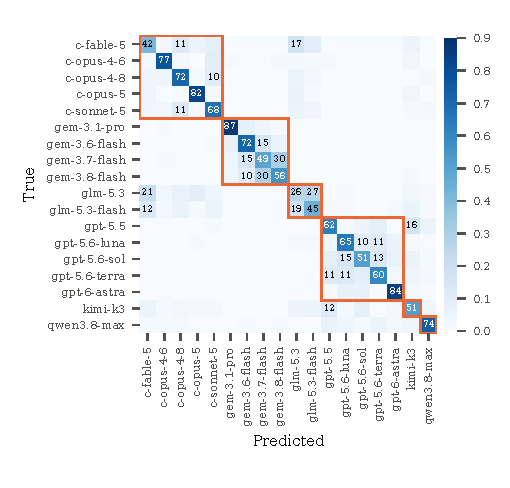
\includegraphics[width=\linewidth]{figures/fig_confusion.pdf}
\caption{Row-normalised confusion matrix (\%) of the Qwen3-8B LoRA24 model, outer folds of both partitions. Orange boxes mark providers. Nearly all mass lies inside the boxes. The large off-block cells are \texttt{glm-5.3}$\to$\texttt{claude-fable-5} and the reverse.}
\label{fig:confusion}
\end{figure}

\begin{figure*}[t]
\centering
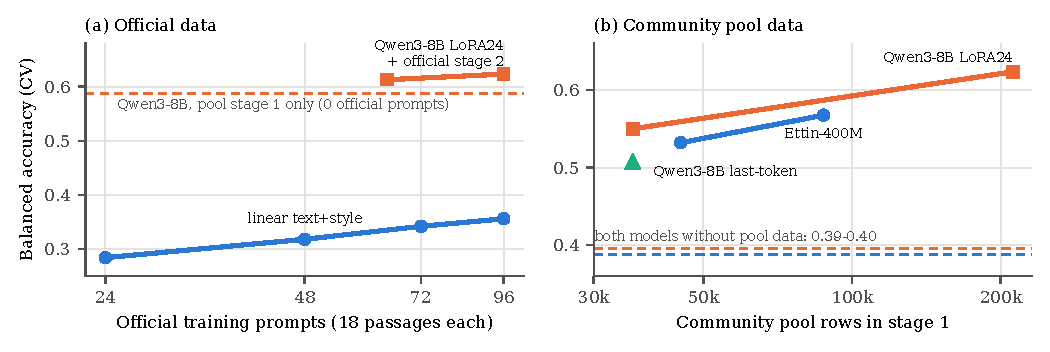
\includegraphics[width=0.92\linewidth]{figures/fig_scaling.pdf}
\caption{Scaling evidence. (a) BA vs number of official training prompts: the linear model gains about +0.036 per doubling with no sign of flattening, and the 8B about +0.018. (b) BA vs community-pool rows used in stage 1. Doubling pool data gave +0.036 to the encoder; 36k$\to$212k rows gave +0.073 to the 8B. Without pool data both models sit at 0.39--0.40 (dashed).}
\label{fig:scaling}
\end{figure*}

\subsection{Performance of the proposed solution}

\begin{table}[t]
\centering\small
\caption{Two-stage models (nested CV). ``Stage 1'' is the pool model alone. Pool data and the LoRA24 recipe give the large steps.}
\label{tab:models}
\begin{tabular}{lccc}
\toprule
Model & pool rows & p0 & p1 \\
\midrule
Ettin-400M, official only & 0 & 0.388 & -- \\
Ettin-400M, stage 1 only & 45k & 0.523 & 0.523 \\
Ettin-400M, stage 1+2 & 45k & 0.530 & 0.534 \\
Ettin-400M, stage 1+2 & 88k & 0.566 & 0.569 \\
Ettin-1B, stage 1+2 & 27k & 0.517 & 0.522 \\
\midrule
Qwen3-8B last-token, official only & 0 & 0.396 & -- \\
Qwen3-8B last-token, stage 1+2 & 36k & 0.507 & 0.508 \\
Qwen3-8B LoRA24, stage 1+2 & 36k & 0.550 & -- \\
Qwen3-8B LoRA24, stage 1 only & 212k & 0.588 & 0.588 \\
\textbf{Qwen3-8B LoRA24, stage 1+2} & \textbf{212k} & \textbf{0.623} & \textbf{0.624} \\
Qwen3-14B LoRA24, stage 1+2 & 167k & 0.609 & 0.621 \\
\bottomrule
\end{tabular}
\end{table}

Table~\ref{tab:models} gives the main results.
\begin{itemize}
\item \textbf{Pool pre-training is the biggest lever}: +0.142 [+0.119, +0.166] for the same Ettin-400M (p0). Doubling the pool (2.5k$\to$5k rows per label) adds +0.036 on both partitions (Fig.~\ref{fig:scaling}b).
\item \textbf{Model size alone does not help.} On official data the 8B ties Ettin-400M at $\sim$30$\times$ the cost. Ettin-1B trails the 400M by 0.013, about the same as the seed-to-seed spread.
\item \textbf{The LoRA24 recipe} adds +0.043 [+0.025, +0.062] to the 8B at equal data. Training it on the whole pool adds another +0.073. The final 8B beats our best five-model ensemble by +0.039 / +0.028, with intervals clear of zero, and is our best single model.
\item \textbf{Stage~2 on official rows still pays}: +0.035 over stage~1 alone for the 8B.
\end{itemize}
On the locked confirmation set (30 unseen prompts, scored once), the final 8B trained on all 120 development prompts scores \textbf{0.633} [0.600, 0.665], consistent with nested CV.

\begin{table}[t]
\centering\small
\caption{Soft centring of the 8B's logits within content clusters, with prompts subsampled to $m$ answers (5 draws). BA plain $\to$ centred.}
\label{tab:centring}
\begin{tabular}{ccc}
\toprule
$m$ & p0 & p1 \\
\midrule
2 & 0.611$\to$0.621 & 0.622$\to$0.622 \\
3 & 0.620$\to$0.628 & 0.611$\to$0.636 \\
6 & 0.624$\to$0.640 & 0.628$\to$0.648 \\
18 & 0.623$\to$0.646 & 0.624$\to$0.647 \\
\midrule
\multicolumn{3}{l}{confirmation set: +0.004 ($m$=18), $-$0.005 ($m$=2), CIs span 0} \\
\multicolumn{3}{l}{public leaderboard: 0.599 $\to$ \textbf{0.619}} \\
\bottomrule
\end{tabular}
\end{table}

\paragraph{Test-time centring (Table~\ref{tab:centring}).} The gain grows with answers per prompt, as expected. With $m=2$, the reported layout of the test, it is small and uncertain. On the confirmation set it was about zero, but on the public leaderboard it added +0.020. This mixed evidence is itself a finding (\S\ref{sec:why}).

\subsection{Leaderboard results}

\begin{figure*}[t]
\centering
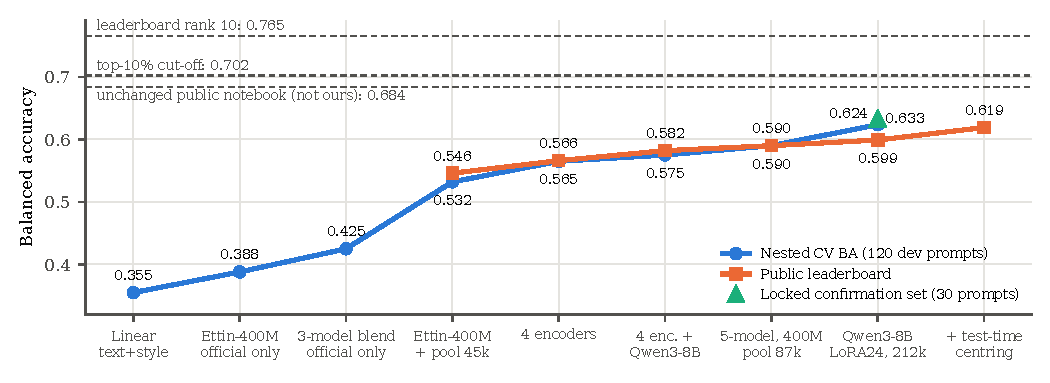
\includegraphics[width=0.95\linewidth]{figures/fig_progress.pdf}
\caption{Progress over the project: nested CV (mean of the two partitions) and public leaderboard for each milestone. CV ordered every submission the same way as the leaderboard; the gap widened only for the strongest single model, whose LB (0.599) is 0.024 below its CV. The dashed lines are \emph{reference points}, not our results.}
\label{fig:progress}
\end{figure*}

\begin{table}[t]
\centering\small
\caption{All Kaggle submissions (public LB, 40\% of test). The last two rows fork a public community notebook and are reported as a reference, not as our method.}
\label{tab:lb}
\begin{tabular}{p{4.7cm}cc}
\toprule
Submission & CV p0/p1 & LB \\
\midrule
Ettin-400M + pool & .530/.534 & 0.546 \\
Ettin-400M$\times$3 + Ettin-1B & .568/.562 & 0.566 \\
+ Qwen3-8B (last-token) & .575/.575 & 0.582 \\
400M (88k pool) replaces a seed & .584/.596 & 0.590 \\
Qwen3-8B LoRA24, 212k pool & .623/.624 & 0.599 \\
\textbf{same + test-time centring} & -- & \textbf{0.619} \\
\midrule
public 0.684 notebook, unchanged & -- & 0.684 \\
same + our 8B as 7th member & -- & 0.680 \\
\bottomrule
\end{tabular}
\end{table}

Figure~\ref{fig:progress} and Table~\ref{tab:lb} track all eight submissions. CV and the leaderboard ordered our five model submissions identically, and agreed within 0.015 up to the 8B, whose LB fell 0.024 below its CV. Our own best is \textbf{0.619}. On 12 Nov we forked the strongest public notebook (an ensemble of six LoRA decoders and other stages by community authors~\cite{kaggle_public684}) to use as a base for our additions. It reproduced its published 0.684 exactly. Adding our 8B as a seventh member gave 0.680, inside the leaderboard's noise, so our model brings nothing that ensemble lacks. As of 20~Nov~2026 (Fig.~\ref{fig:screenshot}) the team's leaderboard entry is that unchanged fork: 0.684, rank 1,595 of 6,529 (top 25\%). Our own pipeline's 0.619 would rank about 3,260th. The top-10\% cut-off is 0.702, and tenth place is 0.765. Public notebooks keep rising: by 19 Nov the best one scored 0.704~\cite{kaggle_704}, and on 20 Nov 570 teams were tied at exactly 0.702, the score of the latest version of the public ensemble we forked.

\begin{figure*}[t]
\centering
\begin{minipage}[t]{0.485\textwidth}\centering
\fbox{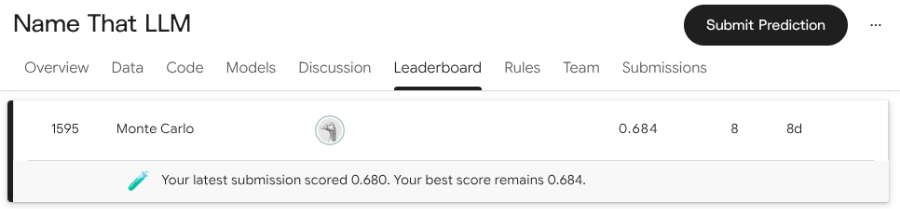
\includegraphics[width=0.97\linewidth]{figures/kaggle_leaderboard.png}}\\[2pt]
{\small (a) Public leaderboard, team \emph{Monte Carlo}: rank 1,595 of 6,529.}
\end{minipage}\hfill
\begin{minipage}[t]{0.485\textwidth}\centering
\fbox{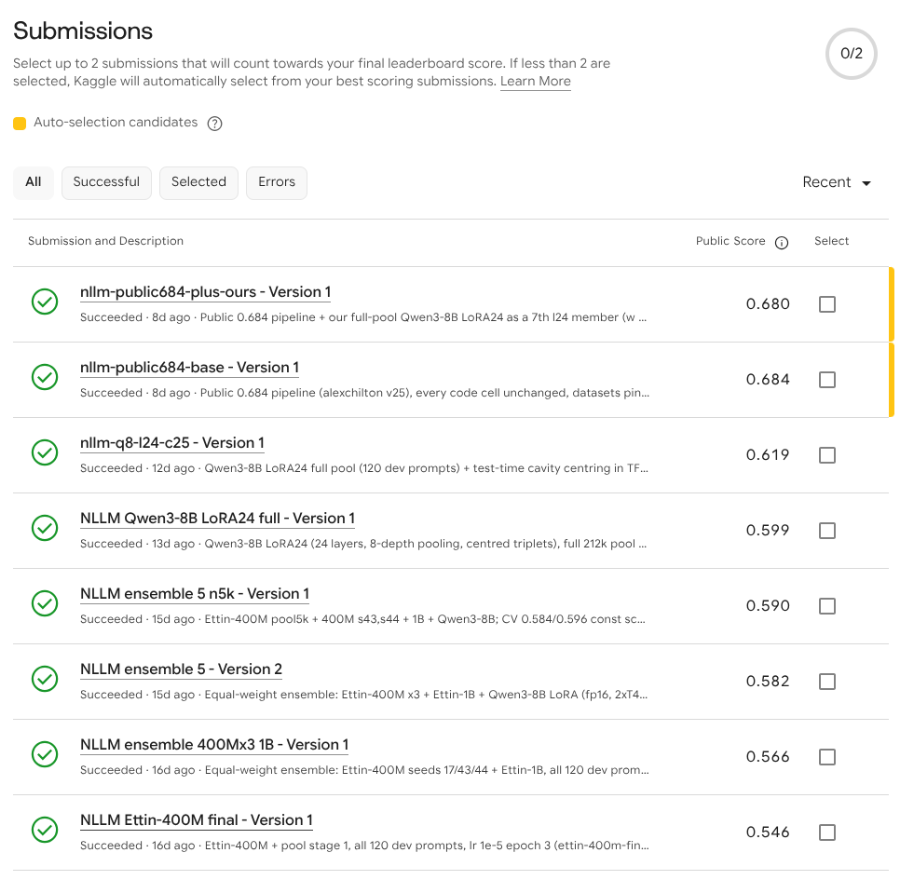
\includegraphics[width=0.97\linewidth]{figures/kaggle_submissions.png}}\\[2pt]
{\small (b) Our eight submissions and their public scores.}
\end{minipage}
\caption{Kaggle screenshots taken on 20 Nov 2026. The best score (0.684) is the unchanged public notebook; our own best model submission is 0.619 (\texttt{nllm-q8-l24-c25}). Scores match Table~\ref{tab:lb}.}
\label{fig:screenshot}
\end{figure*}

\subsection{Do sibling specialists help? (Exp.~12)}
\label{sec:specialists}

\begin{table}[t]
\centering\small
\caption{Exp.~12. Top: pairwise AUC between siblings, from the 8B's scores and from a dedicated within-group specialist (outer folds, mean of partitions). Bottom: paired $\Delta$BA when the specialist redistributes the 8B's probability inside its group ($\alpha$ chosen on inner folds).}
\label{tab:specialists}
\begin{tabular}{lcc}
\toprule
Sibling pair & 8B & specialist \\
\midrule
\texttt{gemini-3.7} vs \texttt{3.8} & 0.654 & 0.623 \\
\texttt{gemini-3.6} vs \texttt{3.7} & 0.860 & 0.803 \\
\texttt{glm-5.3} vs \texttt{glm-5.3-flash} & 0.632 & 0.527 \\
\texttt{claude-fable-5} vs \texttt{glm-5.3} & 0.695 & 0.530 \\
\texttt{gpt-5.6-luna} vs \texttt{sol} & 0.868 & 0.724 \\
\texttt{gpt-5.6-sol} vs \texttt{terra} & 0.873 & 0.732 \\
\texttt{claude-opus-4-8} vs \texttt{sonnet-5} & 0.919 & 0.832 \\
\midrule
Added to the 8B & $\Delta$ p0 & $\Delta$ p1 \\
\midrule
Claude specialist & $-$0.001 & $-$0.002 \\
Gemini specialist & +0.001 & $-$0.001 \\
GPT specialist & +0.002 & +0.002 \\
GLM specialist ($\alpha=0$ in 10/10 folds) & 0.000 & 0.000 \\
fable/GLM triangle specialist & $-$0.000 & $-$0.004 \\
all four families & +0.002 & $-$0.001 \\
\bottomrule
\end{tabular}\\[2pt]
{\footnotesize Every $\Delta$ interval spans zero; all four families: [$-$0.005, +0.009] / [$-$0.010, +0.006].}
\end{table}

Since most errors are confusions between siblings, we tested the obvious remedy: a model trained \emph{only} to tell siblings apart. For each group (Claude, Gemini, GPT, the GLM pair, and the cross-family \texttt{claude-fable-5}/GLM triangle) we trained a text+style linear specialist on that group's labels only. Its training data was the official rows of the fit's training prompts plus 2,000 pool rows per label, the same rows the 8B's stage~1 drew from. The specialist may only redistribute the 8B's probability \emph{inside} its group:
\[
p(l) = p_{8B}(G)\cdot\mathrm{softmax}_{G}\big(z_{8B,G} + \alpha\, s_G\big)_l, \quad l\in G,
\]
where $s_G$ is the specialist's standardised score and $\alpha\in[0,12]$ is chosen per outer fold on inner OOF 18-class BA ($\alpha=0$ is the 8B unchanged). The protocol is fully nested: 200 fits on both partitions, CPU only.

Table~\ref{tab:specialists} gives a clear negative. The specialist is a \emph{worse} sibling classifier than the 18-way 8B on every hard pair, and on the GLM pair and the triangle it is at chance (AUC 0.46--0.53). Inner selection set $\alpha=0$ in all ten folds for GLM and in seven of ten for the triangle. Every combined $\Delta$ is between $-$0.004 and +0.002, with intervals spanning zero. The 8B's softmax is already a within-family classifier, trained with the same loss on the same rows, so a specialist on the same data gains focus but no new information. What \emph{did} move the GLM pair was new evidence: the real GLM-5.3-Flash likelihood (\S\ref{sec:negative}) raised \texttt{glm-5.3} recall from 0.24 to 0.40.

\subsection{Is there a word-choice signal between siblings? (Exp.~13)}
\label{sec:words}

\begin{table}[t]
\centering\small
\caption{Exp.~13, prompt-paired on official data. Sig.: tokens with $q<0.10$ (McNemar, Benjamini--Hochberg). Split: sign agreement of each pair's top 20 tokens across random halves of the prompts (a within-prompt label swap gives 0.42--0.48). Twin: given both answers to one prompt, how often the right one is picked by words + style (AUC, 10-fold over prompts) and by the 8B (accuracy, dev prompts).}
\label{tab:siblingwords}
\setlength{\tabcolsep}{3pt}
\begin{tabular}{lcccc}
\toprule
Pair & Sig. & Split & \multicolumn{2}{c}{Twin} \\
 & & & words+style & 8B \\
\midrule
\texttt{opus-5} vs \texttt{sonnet-5} & 46 & 0.88 & 0.99 & 1.00 \\
\texttt{gemini-3.1-pro} vs \texttt{3.8} & 49 & 0.93 & 0.99 & 1.00 \\
\texttt{gpt-5.5} vs \texttt{6-astra} & 19 & 0.86 & 0.99 & 1.00 \\
\midrule
\texttt{gemini-3.6} vs \texttt{3.7} & 0 & 0.58 & 0.79 & 0.94 \\
\texttt{gpt-5.6-luna} vs \texttt{sol} & 0 & 0.52 & 0.75 & 0.91 \\
\texttt{gpt-5.6-sol} vs \texttt{terra} & 0 & 0.49 & 0.70 & 0.91 \\
\texttt{gemini-3.7} vs \texttt{3.8} & 0 & 0.61 & 0.66 & 0.70 \\
\texttt{glm-5.3} vs \texttt{-flash} & 0 & 0.50 & 0.57 & 0.64 \\
\texttt{fable-5} vs \texttt{glm-5.3} & 0 & 0.46 & 0.55 & 0.77 \\
\bottomrule
\end{tabular}
\end{table}

Table~\ref{tab:words} shows that word choice separates providers and model generations. We asked whether it also separates the close siblings we confuse. We used the 18~Nov release of the community pool (231k passages).

\textbf{Across sources.} For the hard pairs, the words that separate siblings in the pool do not carry over to official text. Not one of the pool's top 80 tokens is confirmed for Gemini 3.7 vs 3.8, the GLM pair or \texttt{claude-fable-5} vs \texttt{glm-5.3}, and their direction agrees only 44--49\% of the time, a coin flip. As a classifier, word choice is real but redundant. A logistic regression on the pool's 1,000 most common words plus sentence openers, trained on pool rows only, reaches 0.322 BA on official text; all words and word pairs reach 0.363, typography alone 0.225, and words plus typography 0.370 (family right on 68\%). Mixed into the 8B with nested weights, every variant changes BA by $-$0.007 to $-$0.001, with most intervals spanning zero.

\textbf{Within official data, prompt-paired.} Every official prompt is answered by both siblings, so comparing the two answers to the same prompt removes topic entirely. Table~\ref{tab:siblingwords} shows two kinds of sibling. Different generations or tiers differ in dozens of words, and a small word model tells them apart almost perfectly. Close siblings (Gemini 3.6/3.7/3.8, the GPT-5.6 trio, the GLM pair) show \emph{no} significant word. For Gemini 3.7 vs 3.8, 293 tokens had enough data to test, and two reached $p<0.01$ where about three are expected by chance. The only consistent differences are length and rhythm. 3.7 writes slightly longer passages (median 101 vs 84 words, $p=0.009$) with longer sentences (22.9 vs 21.5 words, $p=0.003$) and slightly less varied vocabulary (type--token ratio over the first 60 words 0.886 vs 0.900, $p=0.005$). All three point the same way in 2,782 matched pool pairs (same prompt, same source), although there the length gap disappears. Even with both answers to the same prompt, words and style pick the 3.7 answer with AUC only 0.66. For the GLM pair and fable vs GLM, no word and no style measure is significant at $p<0.01$, and split-half agreement is at the swap level. On every hard pair the 8B does better than words and style, so whatever separates those siblings is not a choice of words.

\subsection{What did not work}
\label{sec:negative}
The protocol was just as useful for rejecting ideas. All results are paired against the relevant baseline:
\begin{itemize}
\item \textbf{Generative classifier} (one label-conditioned LM, likelihood ratio): 0.280 vs 0.530. The likelihood mostly measures how predictable the content is.
\item \textbf{Sibling-drawn training units} (put confusable labels in the same prompt triplet): $-$0.008 [$-$0.018, +0.002].
\item \textbf{Up-weighting our best-matched (Codex) answers $5\times$}: +0.002 / $-$0.005. \textbf{Extra CC-BY sources}: +0.009 / $-$0.007.
\item \textbf{More seeds}: a third Ettin-400M seed adds +0.002 / +0.012. A second Ettin-1B seed adds $-$0.010 / +0.005, with the sign flipping between partitions.
\item \textbf{Distinct-label assignment within prompt groups}: +0.000 at $m=2$ (but +0.15 at $m=18$, a trap of 18-answer CV).
\item \textbf{Post-hoc corrections of the 8B's saved scores} (nested, $\lambda$ chosen on inner folds). Transductive EM, which refits class Gaussians in logit space on the held-out rows: $-$0.009 / $-$0.007 with 18 answers per prompt and $-$0.011 / $-$0.017 with 2. A soft prior against punctuation marks a label never used in training (a public-notebook trick): +0.0005 / +0.0005, changing three rows. Priors on word count, sentence count or words per sentence: $-$0.005 to 0.000.
\item \textbf{Hidden states of the real GLM-5.3} (public weights, 54 of 78 layers): +0.001 / $-$0.005.
\item \textbf{Likelihood under the real GLM-5.3-Flash} (public 117\,GB quantised weights, streamed layer by layer on the 16\,GB GPU), with a neutral reference LM to remove content predictability as in Fast-DetectGPT~\cite{bao2024fastdetectgpt}. This one \emph{helped}: +0.016 [+0.005, +0.027] / +0.017 [+0.006, +0.029], with \texttt{glm-5.3} recall 0.24$\to$0.40. We could not deploy it, because the notebook would have to stream 117\,GB of weights inside the time budget.
\end{itemize}

%=====================================================================
\section{Why we could not improve further}
\label{sec:why}

\begin{figure}[t]
\centering
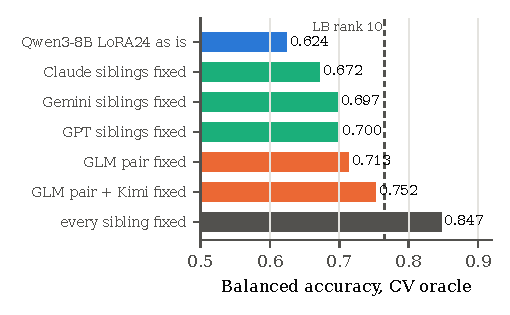
\includegraphics[width=\linewidth]{figures/fig_headroom.pdf}
\caption{Oracle analysis of the 8B's CV predictions: BA if one group of confusions were resolved perfectly, all else unchanged. The three open-weight labels (GLM pair, Kimi) hold more error than any closed family.}
\label{fig:headroom}
\end{figure}

Our CV rose from 0.355 to 0.623 within the first week (2--7 Nov). The following week of experiments (centring, a 14B backbone, sibling-aware training, real-model features, a fork of the public ensemble) moved our own submitted model by at most +0.02. We identify five causes, each backed by measurements.

\paragraph{1. The remaining error is sibling confusion, and part of it is near-irreducible from text.} The 8B predicts the correct \emph{family} on 84.7\% of rows. Given a correct family, the exact model is right only 73.7\% of the time. Three groups hold 47\% of all errors (Fig.~\ref{fig:confusion}): Gemini 3.6/3.7/3.8, the GPT-5.5/5.6 variants, and the \texttt{claude-fable-5}/GLM triangle. Short passages are much harder: accuracy rises from 0.45 for 36--59 words to 0.76 for 170--274 words. For Gemini 3.7 vs 3.8, a classifier trained only on matched community pairs reaches an AUC of just 0.59, and the 3.7 model can no longer be queried. The ceiling here is set by the data, not the model. Official rows do not help this pair at all: its AUC is 0.657 after pool-only stage~1 and 0.653 after official stage~2, whereas stage~2 does lift the GLM pair (0.580$\to$0.631). Stage~2 mostly \emph{trades} recall between siblings rather than separating them: \texttt{gemini-3.7} gains 0.10 while 3.8 loses 0.08. A dedicated specialist (Exp.~12, Table~\ref{tab:specialists}) confirms this. Trained only to separate siblings, on the same official and pool rows, it is worse than the 8B on every hard pair and at chance on the GLM pair, and mixing it in changes BA by $-$0.004 to +0.002. Word choice does not separate them either (Exp.~13). Close siblings show no significant word difference even between two answers to the same prompt, and Gemini 3.7 and 3.8 differ only slightly in length and sentence length. Fig.~\ref{fig:headroom} shows where the headroom is. Perfect handling of the GLM pair and Kimi alone would lift our 8B to 0.752, roughly the top ten.

\paragraph{2. The bottleneck is official-like data, and we could not produce it.} Every large step in Fig.~\ref{fig:progress} came from data: +0.14 from the pool, +0.036 per pool doubling, +0.073 from the full pool on the 8B. Architecture changes, a 14B backbone (0.609 / 0.621) and sibling-aware training did not move the curve. The pool is now used in full (212k rows), so more of it is not available. Our own collection did not match the hosts' setup (Kimi and Qwen recognition 0.01--0.02, every source too long), and match-weighting cannot fix differences in content or habits. Official rows are the most valuable rows: one is worth about 40 pool rows on the 8B's curves. The top teams report that ``nearly all'' of their single-model gain (0.65--0.68 vs our 0.62) came from their own generated data. Matching each model's exact serving setup is a data-engineering problem we only partly solved.

\paragraph{3. Ensembles saturate because the members share data.} Equal-weight encoder blends flattened at 0.565--0.570. Seeds added 0.002--0.012 each, and a stronger member trained on the same data (LoRA24 at 36k rows) added nothing to the blend because it agreed with the existing members on 60\% of rows. The public leaderboard tells the same story: our 8B inside the public ensemble scored 0.680 vs 0.684, and that ensemble's own authors measured at most $\pm$0.004 per extra member of the same kind. Diversity must come from \emph{different evidence} (other data views, the real models' likelihoods), not from more members.

\paragraph{4. CV and the leaderboard measure different things.} Our CV groups have 18 answers per prompt; the test reportedly has about two. Any method that uses prompt structure (centring, assignment) is therefore overestimated in CV, by up to +0.15 for assignment, as the community found out the hard way. The 8B is the clearest case: CV 0.623, confirmation 0.633, public LB 0.599. The public split, then, has a harder class mix or harder prompts than both of our splits. Centring was $\approx$0 on the confirmation set but +0.020 on the LB. With $\pm$0.009 noise between identical submissions and the public split covering only 40\% of the test, differences below about 0.01 cannot be resolved on the leaderboard. We deliberately did not tune to it, given five submissions a day and a private split with a different class mix.

\paragraph{5. Compute and time.} One nested 8B run takes about 5\,h on our single shared L40S (a 14B run needs two jobs). The most promising remaining direction is real-model likelihood for the open-weight labels, worth +0.035 out-of-fold in a public notebook~\cite{kaggle_glm} and +0.016 in our study. It requires streaming 117--730\,GB quantised models (GLM-5.3-Flash, GLM-5.3, Kimi K3) layer by layer. Our GLM-5.3 run stopped at layer 54 of 78. A Kimi K3 stage would need an estimated 2--3\,h of the 9\,h notebook limit, which the base ensemble already fills. The workstation could not keep running such jobs, so we stopped local LLM runs on 14~Nov. We also lost time on our original last-token decoder recipe, which trailed the community recipe by 0.06--0.08 until we adopted the latter on 6 Nov. Finally, holding out 30 prompts for confirmation cost the final models about 0.01. We accepted that cost so as to have one unbiased estimate.

%=====================================================================
\section{Conclusion}
\label{sec:conclusion}

We framed exact LLM attribution as prompt-shift classification, built a nested prompt-grouped protocol, and used it to raise our own pipeline from 0.355 to 0.623 CV BA (0.633 on locked prompts, 0.619 public LB). The headline lesson is that \textbf{data beat models}: training on 212k community passages, reweighted to official statistics, was worth more than any architecture choice. Our analysis shows that the remaining error is dominated by sibling models, which neither better text classifiers, dedicated sibling specialists nor word-choice features separate.

\paragraph{What we learned.}
\begin{enumerate}[label=(\roman*)]
\item \emph{Validation design decides what you learn.} Nested, prompt-grouped CV with paired prompt bootstraps let us reject ideas worth $\pm$0.01 that the noisy leaderboard could not resolve, and it ordered all five of our model submissions the same way the leaderboard did. It still could not mimic the test's sparse prompt groups, so the protocol should have subsampled answers per prompt from the start.
\item \emph{Respect the signal.} Raw typography carries real information, so normalising text would have discarded it.
\item \emph{Data provenance is a modelling problem.} The same model served through another route is, for this task, a different class.
\item \emph{Read the field early.} The community's LoRA24 recipe and pool were worth more than our own architecture search.
\item \emph{Ensembles need different evidence}, not more of the same model.
\item \emph{Fingerprints are hierarchical.} Providers differ in typography and word choice, and model generations differ in word choice. Close siblings differ in neither, which is exactly where our errors are.
\end{enumerate}

\paragraph{Future work.} (a) \emph{Kimi first.} Classifying \texttt{kimi-k3} perfectly would add +0.039 / +0.040 to the 8B, and +0.024 / +0.026 even if only the 15\% of rows with the highest predicted Kimi probability were corrected. The pool's 18~Nov release tags each row's reasoning setting, and only Kimi rows generated with ``high'' effort look official to the pool's own fidelity measure (0.81, against 0.11--0.34 for every other setting). In a quick check (a linear model trained on pool rows only and tested on all official rows; not nested, so optimistic), keeping only the official-like Kimi sources raised Kimi recall from 0.11 to 0.34 against 0.09 for a same-size random subset. BA rose by +0.007, although the other labels together lost 0.006. Two experiments follow: a stage~1 that keeps only those Kimi rows, and a Kimi K3 likelihood stage, contrasted against GLM-5.3-Flash and applied only to rows with high Kimi probability. (b) Generate official-like data label by label, using our closeness instrument as an acceptance gate, starting with Qwen and GLM, where community sources are weakest. (c) Add the GLM-5.3 vs GLM-5.3-Flash likelihood contrast inside the notebook's time budget. (d) Retrain final members on all 150 prompts.

\paragraph{Acknowledgements.} We build on public Kaggle work: the Open Pool dataset, the LoRA24 decoder recipe, the 0.684 ensemble notebook and the GLM likelihood stage~\cite{kaggle_pool,kaggle_lora24,kaggle_public684,kaggle_glm}. The NTU TC2 cluster provided the L40S GPU.

\small
\begin{thebibliography}{99}\setlength{\itemsep}{0pt}
\bibitem{bao2024fastdetectgpt} G.~Bao, Y.~Zhao, Z.~Teng, L.~Yang, Y.~Zhang. Fast-DetectGPT: Efficient zero-shot detection of machine-generated text via conditional probability curvature. \emph{ICLR}, 2024.
\bibitem{brodersen2010} K.~H.~Brodersen, C.~S.~Ong, K.~E.~Stephan, J.~M.~Buhmann. The balanced accuracy and its posterior distribution. \emph{ICPR}, 2010.
\bibitem{efron1993} B.~Efron, R.~J.~Tibshirani. \emph{An Introduction to the Bootstrap}. Chapman \& Hall, 1993.
\bibitem{hu2022lora} E.~J.~Hu, Y.~Shen, P.~Wallis, Z.~Allen-Zhu, Y.~Li, S.~Wang, L.~Wang, W.~Chen. LoRA: Low-rank adaptation of large language models. \emph{ICLR}, 2022.
\bibitem{kaggle_lora24} L.~Boesen. name-that-llm-train-lora24-s7 (Kaggle notebook), Oct.~2026. \url{https://www.kaggle.com/code/lucasboesen/name-that-llm-train-lora24-s7}; and N.~Dahal. Two-stage LoRA on the public pool (Kaggle notebook), Oct.~2026. \url{https://www.kaggle.com/code/nishantdahal/two-stage-lora-on-the-public-pool}
\bibitem{kaggle_pool} Kaggle user \texttt{crtproduction}. Name That LLM Open Pool (Kaggle dataset, CC~BY-SA~4.0), v13 (3~Nov.~2026) and the 18~Nov.~2026 release. \url{https://www.kaggle.com/datasets/crtproduction/name-that-llm-open-pool}
\bibitem{kaggle_glm} J.~Padilla. 0.689 | Real GLM-5.3 Likelihood on 2xT4 (Kaggle notebook), Nov.~2026. \url{https://www.kaggle.com/code/estopadilla/0-689-real-glm-5-3-likelihood-on-2xt4}
\bibitem{kaggle_704} Kaggle user \texttt{lightningv08}. 0.704 | GLM Fable Routing + Qwen3.8-27B LoRA (Kaggle notebook), Nov.~2026. \url{https://www.kaggle.com/code/lightningv08/0-704-glm-fable-routing-qwen3-8-27b-lora}
\bibitem{kaggle_public684} A.~Chilton (\texttt{alexchilton}) and contributors. Name That LLM 0.684: All Public + What Failed (Kaggle notebook, version 25; since retitled 0.702), Nov.~2026. \url{https://www.kaggle.com/code/alexchilton/name-that-llm-0-702-all-public-what-failed}
\bibitem{liu2019roberta} Y.~Liu \emph{et al.} RoBERTa: A robustly optimized BERT pretraining approach. arXiv:1907.11692, 2019.
\bibitem{loshchilov2019} I.~Loshchilov, F.~Hutter. Decoupled weight decay regularization. \emph{ICLR}, 2019.
\bibitem{mitchell2023detectgpt} E.~Mitchell, Y.~Lee, A.~Khazatsky, C.~D.~Manning, C.~Finn. DetectGPT: Zero-shot machine-generated text detection using probability curvature. \emph{ICML}, 2023.
\bibitem{stamatatos2009} E.~Stamatatos. A survey of modern authorship attribution methods. \emph{JASIST}, 60(3):538--556, 2009.
\bibitem{uchendu2020} A.~Uchendu, T.~Le, K.~Shu, D.~Lee. Authorship attribution for neural text generation. \emph{EMNLP}, 2020.
\bibitem{varma2006} S.~Varma, R.~Simon. Bias in error estimation when using cross-validation for model selection. \emph{BMC Bioinformatics}, 7:91, 2006.
\bibitem{warner2024modernbert} B.~Warner \emph{et al.} Smarter, better, faster, longer: A modern bidirectional encoder for fast, memory efficient, and long context finetuning and inference (ModernBERT). arXiv:2412.13663, 2024.
\bibitem{weller2025ettin} O.~Weller \emph{et al.} Seq vs Seq: An open suite of paired encoders and decoders (Ettin). arXiv:2507.11412, 2025.
\bibitem{yang2025qwen3} A.~Yang \emph{et al.} Qwen3 technical report. arXiv:2505.09388, 2025.
\end{thebibliography}

\end{document}
